\chapter{Fundamentação Teórica}
\label{cap:fund}

\section{Definições Principais}

Para melhor esclarecer os assuntos abordados, é importante que seja primeiramente definido alguns dos termos centrais para a fundamentação do trabalho.

\subsection{Qualidade de Serviço}

Qualidade de serviço é uma métrica sistêmica que sumariza o quão bem o sistema provisiona suas funcionalidades em um determinado momento. É possível definir e modelar essa métrica de diversas maneiras, mas para os propósitos deste trabalho, será utilizada uma definição simples que resume a funcionalidade geral numa escala de 0 a 1.

A qualidade de serviço $Q$ do sistema pode ser aproximada pela média ponderada de seus serviços $S_0 ... S_n$ com os pesos de seus fatores de contribuição para a qualidade total $q_0 ... q_n$ \cite{SchedAndOptOfDistributedFT}.

\begin{equation}
    Q = \frac{ \sum^{i = 0}_{n} S_i q_i }{ \sum^{i = 0}_{n} q_i}
\end{equation}
\addEquacao{Qualidade de Serviço}{1}

\subsection{Falhas}

De acordo com a definição de anormalidades de software da IEEE: um erro (\textit{error}) é a diferença entre um valor esperado e o valor obtido. Um defeito (\textit{fault}) é um estado irregular do sistema que pode (ou não) provocar erros que resultem em falhas. Já uma falha (\textit{failure}) é uma incapacidade observável do sistema de cumprir sua função designada, constituindo uma degradação total ou parcial de sua qualidade de serviço \cite{IEEEAnormalities}.

Neste trabalho, o termo "falha" será utilizado de forma mais geral, representando um estado ou evento no sistema que cause uma degradação na sua qualidade de serviço.

\subsubsection{Padrões de Ocorrência}

Falhas podem ser classificadas em 3 grupos principais quanto ao seu padrão de ocorrência \cite{FaultTolerantSystems}.

\begin{itemize}
    \item Falhas Transientes: Ocorrem aleatoriamente e possuem um impacto temporário.

    \item Falhas Intermitentes: Assim como as transientes possuem duração e impacto temporários, porém ocorrem periodicamente.

    \item Falhas Permanentes: Causam uma degradação permanente no sistema da qual não pode ser recuperada, potencialmente necessitando de intervenção externa.
\end{itemize}

\subsection{Dependabilidade}

Será utilizado o termo dependabilidade como uma propriedade que sumariza os atributos:  confiabilidade, disponibilidade, capacidade de manutenção e segurança (conhecidos em inglês como critérios RAMS). Os critérios serão definidos na seção seguinte.

A tolerância à falhas impacta positivamente os critérios confiabilidade e disponibilidade, e pode em alguns casos melhorar a capacidade de manutenção, portanto a tolerância à falhas é um aspecto importante para sistemas com dependabilidade.

\subsubsection{Confiabilidade}

Confiabilidade (\textit{Reliability}), é a probabilidade de um sistema executar corretamente no período $[t_0, t]$. Para modelar essa métrica é necessário um modelo estatístico que é particular da aplicação. A confiabilidade $R$ é uma função do tempo $t$, a taxa de falhas $\lambda$ e quaisquer sejam os outros parâmetros do modelo \cite{FaultInjectionTechniques}.

\begin{equation}
    R(t) = f(t, \lambda, ...)
\end{equation}
\addEquacao{Confiabilidade}{2}

\subsubsection{Disponibilidade}

Disponibilidade (\textit{Availability}) é a razão entre o tempo em que o sistema não consegue prover seu serviço (\textit{downtime}) e o e seu tempo total de operação \cite{FaultInjectionTechniques}. A disponibilidade $A$ pode ser modelada em termos do tempo disponível $t_{up}$ e do tempo indisponível $t_{down}$:

\begin{equation}
    A = t_{up} / (t_{up} + t_{down})
\end{equation}
\addEquacao{Disponibilidade}{3}

\subsubsection{Capacidade de manutenção}

Capacidade de manutenção (\textit{Maintainability}) é a probabilidade de um sistema em um estado inválido ser reparado com sucesso antes de um tempo $t$ \cite{FaultInjectionTechniques}.

A modelagem deste atributo necessita de conhecimento particular sobre a aplicação e sobre a disponibilidade de equipamentos ou especialistas humanos para a realização do reparo. Pode ser definida como uma função probabilidade do tempo $t$, taxa de falhas $\lambda$ e os outros parâmetros do modelo.

\begin{equation}
    M(t) = f(t, \lambda, ...)
\end{equation}
\addEquacao{Capacidade de Manutenção}{4}

\subsubsection{Segurança}

Segurança (\textit{Safety}) é a probabilidade do sistema não causar danos à integridade humana ou à outros patrimônios, independentemente da presença falhas. Por ser um critério muito particular da natureza da aplicação e seu contexto de operação, uma estimativa analítica necessita de um modelo estatístico que não é facilmente sumarizado com apenas uma equação \cite{FaultInjectionTechniques}.

\section{Tolerância à Falhas}

\subsection{Mecanismos de Detecção}

Mecanismos de detecção são responsáveis por identificar a presença de uma falha no sistema, um bom mecanismo de detecção deve ser capaz de detectar uma classe grande de falhas sem introduzir uma penalidade grande ao tempo de execução do sistema. Dentre as possíveis escolhas de mecanismos, os subsequentes são utilizados neste trabalho.

\subsubsection{CRC (Cyclic Redundancy Check)}

Os CRCs são códigos de detecção de erro comumente utilizados em redes de computador e armazenamento não volátil. Para cada segmento de dado é concatenado um valor de checagem que é calculado com base no resto da divisão com um polinômio gerador pré definido \cite{FaultTolerantSystems}.

CRCs são comumente utilizados devido à serem simples de implementar, ocuparem pouco espaço adicional no segmento de dados e serem resilientes à erros em rápida sucessão, falhas transientes que alteram uma região de bits próximos.

\subsubsection{Heartbeat signals}

Os \textit{heartbeat signals} (sinais de batimento cardíaco) são sinais periódicos para garantir a atividade de um nó computacional com o recebimento de uma resposta, são também chamados de \textit{watchdog timers} \cite{DependabilityInEmbeddedSystems}. Uma das aplicações desta técnica em conjunto com reexecução ou replicação é a possibilidade de detectar uma demora excessiva e preventivamente cancelar uma das unidades de execução.

\begin{figure}[H]
    \centering
    \captionsetup{justification=centering}
    \caption{Sequência de um Heartbeat Signal}
    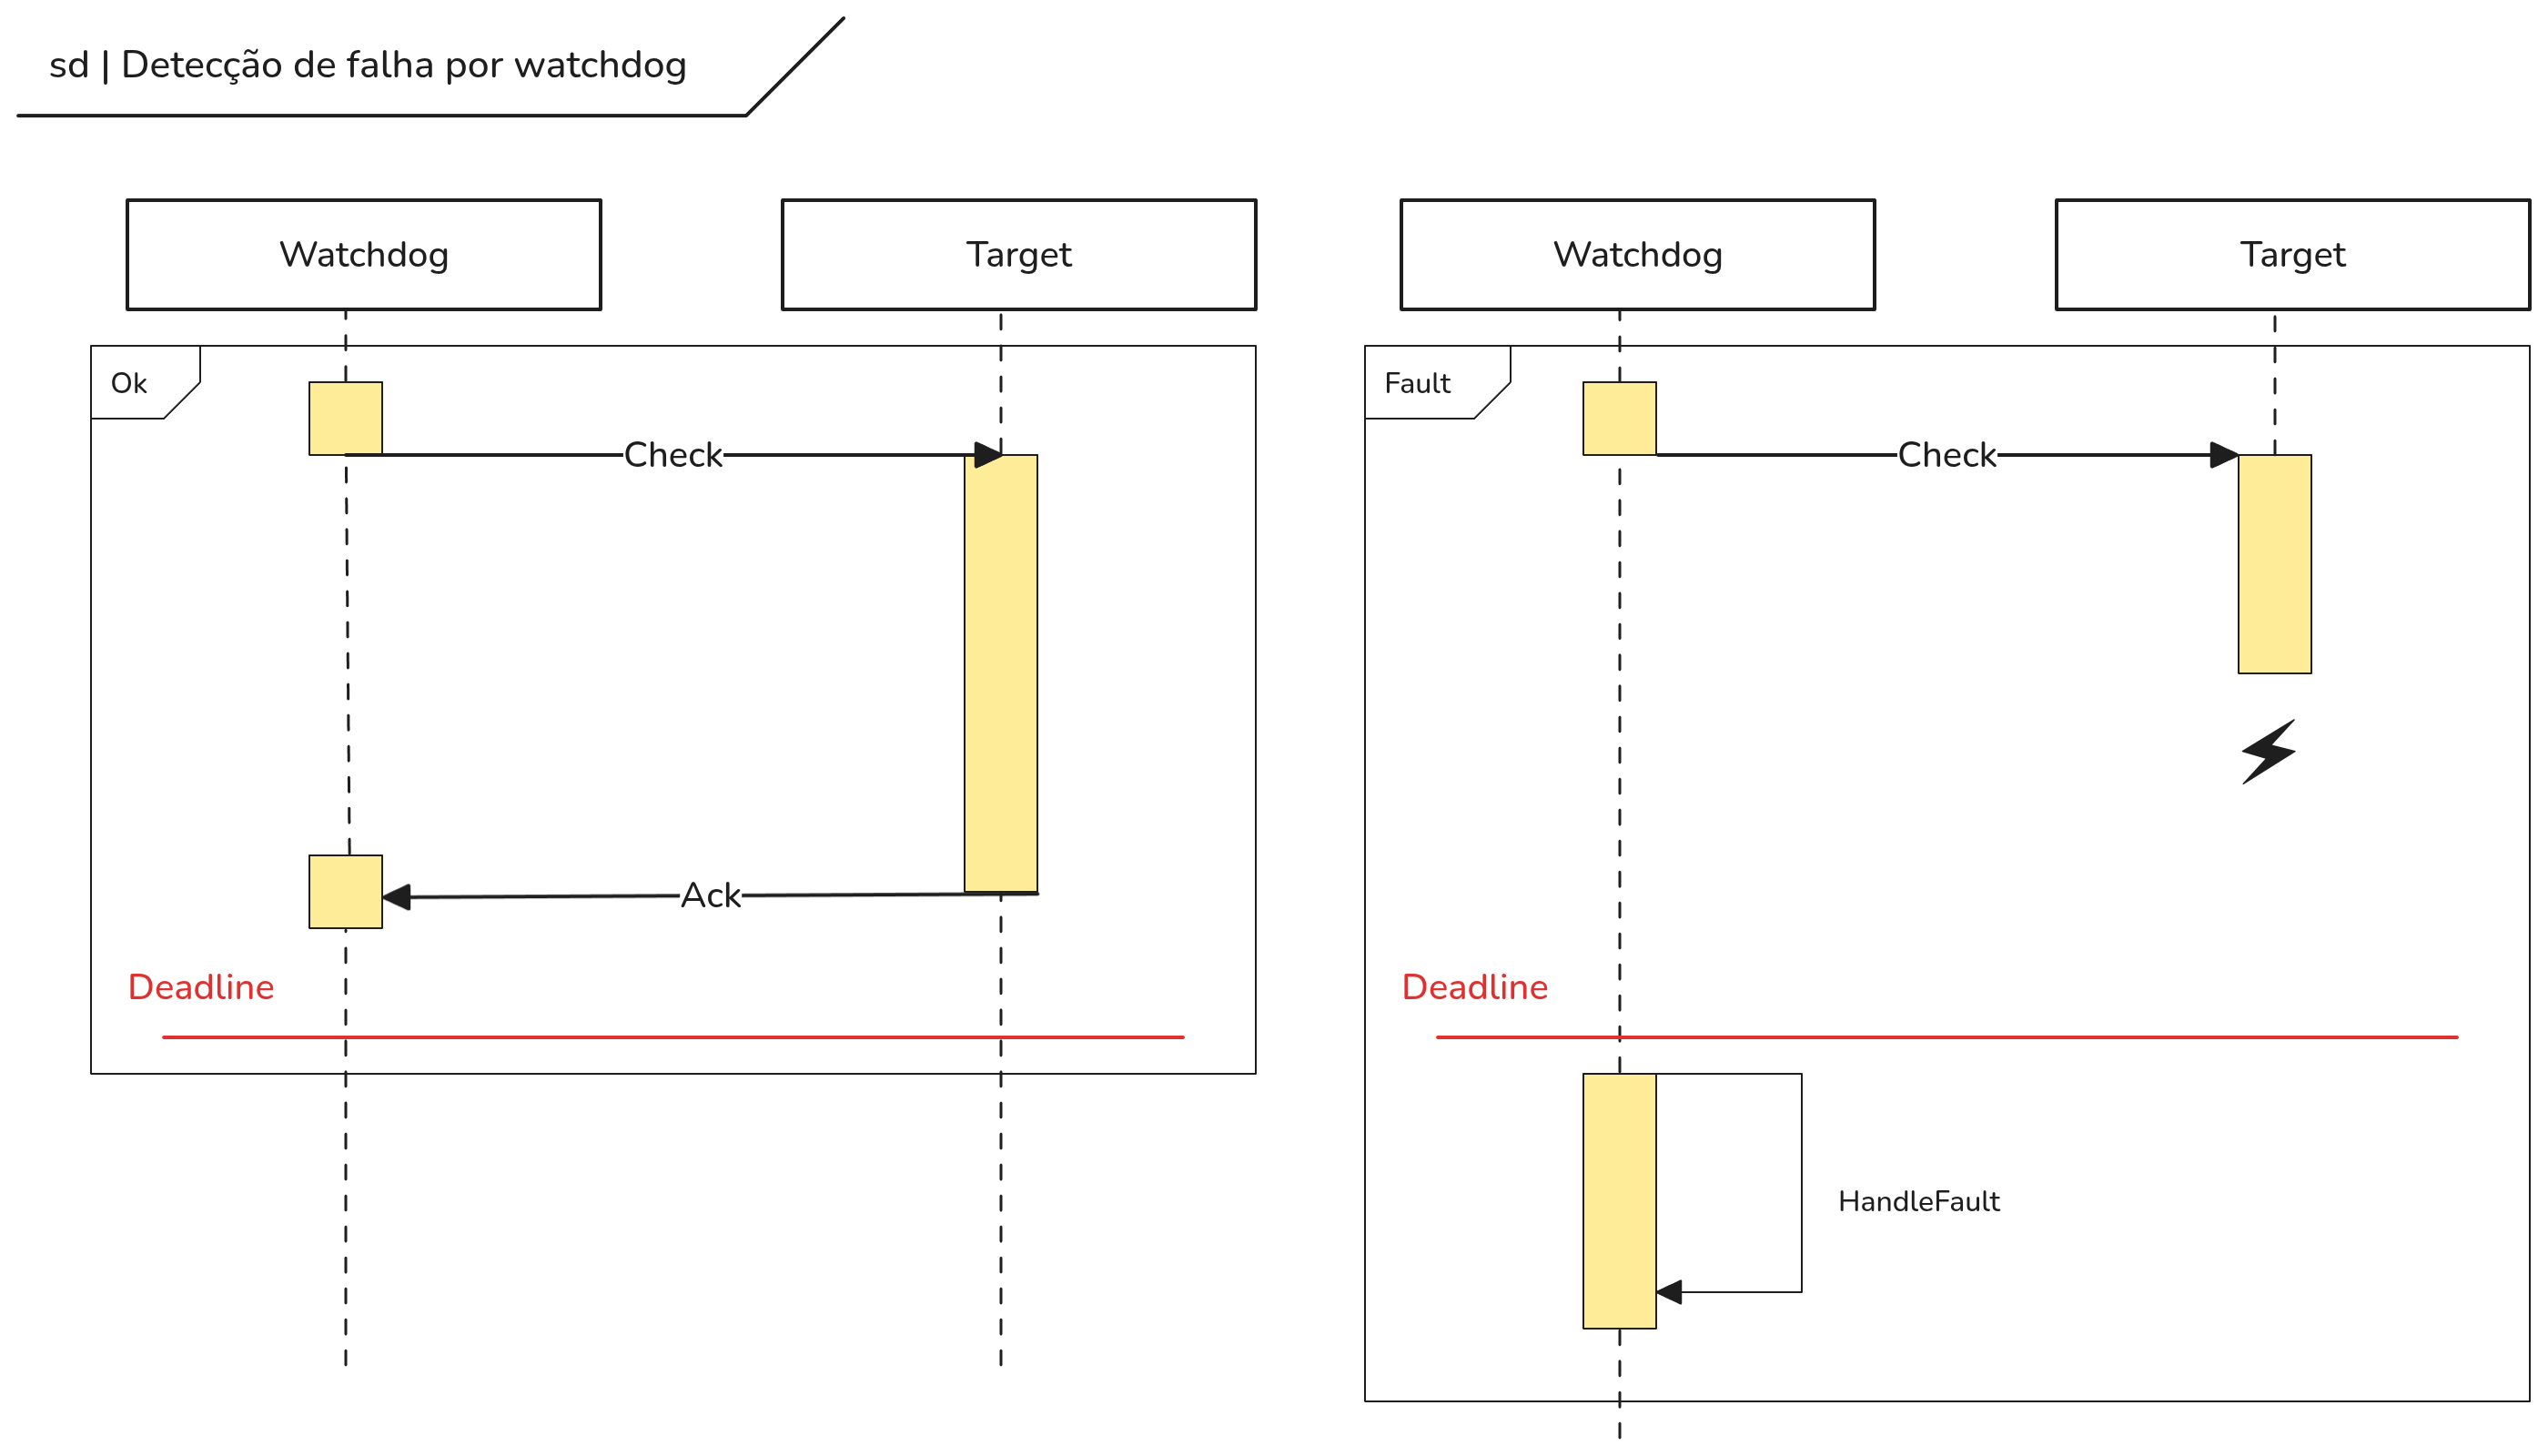
\includegraphics[width=1.0\textwidth]{assets/heartbeat_signal.png}\\
    \captionsetup{justification=raggedright}
    \caption*{Fonte: Elaborada pelo autor}
    \label{fig:heartbeatSignal}
\end{figure}

Na \autoref{fig:heartbeatSignal}, é utilizado a resposta tardia para deduzir a presença de uma falha na tarefa ou no canal de transmissão. Estes sinais também podem ser utilizados no contexto de tempo real para a validação de um prazo ou sub prazo da tarefa \cite{FaultTolerantSystems}.

\subsubsection{Asserts}

Asserts são mecanismos simples e flexíveis para a detecção de falhas, consistindo na verificação de uma condição que, durante uma execução normal do programa, deve permanecer invariavelmente verdadeira (denominada "invariante"). Caso a invariante seja falsa, detecta-se a presença de uma falha. A \autoref{fig:assert} ilustra o fluxo de um assert.

\begin{figure}[H]
    \centering
    \captionsetup{justification=centering}
    \caption{Fluxograma de um Assert}
    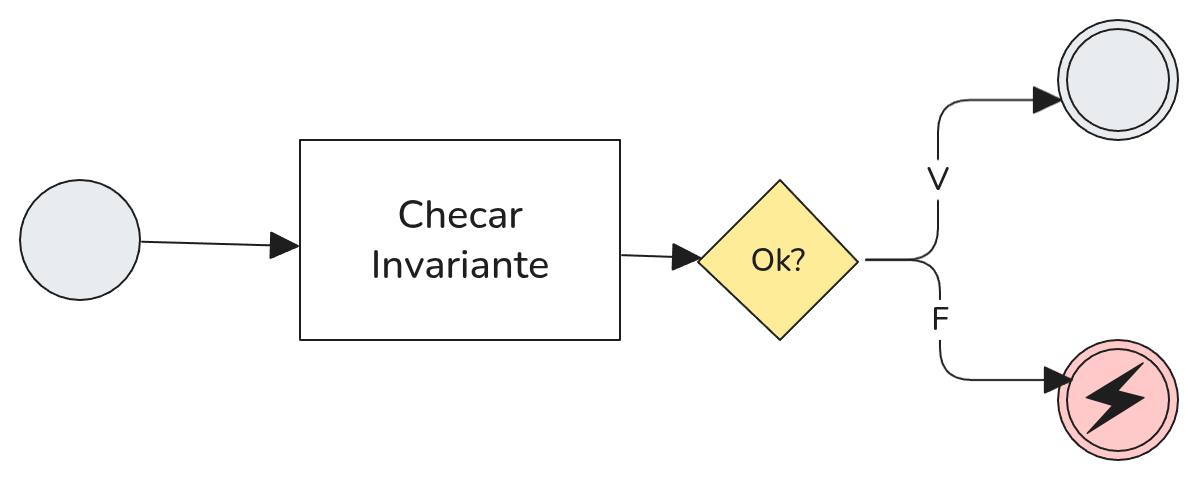
\includegraphics[width=0.5\textwidth]{assets/assert_diagram.png}\\
    \captionsetup{justification=raggedright}
    \caption*{Fonte: Elaborada pelo autor}
    \label{fig:assert}
\end{figure}

Apesar de sua simplicidade, quando usados em conjunto com simulações determinísticas e ferramentas de \textit{fuzzying}, asserts podem detectar erros durante a execução assim como revelar erros de design durante a fase de desenvolvimento \cite{TigerBeetleSafety} \cite{PowerOf10Rules}.

Durante a execução de um sistema tolerante à falhas, asserts servem como uma forma de saber rapidamente que algo errado aconteceu. Porém não são robustos o suficiente para detectar corrupção silenciosa de dados ou pulos inesperados de maneira consistente. Quando asserts são inseridos na entrada ou saída de um procedimento são denominados como pré-condições e pós-condições respectivamente. Alguns compiladores são capazes de automaticamente inserir estas condições para assegurar contratos da interface de um programa. Algumas linguagens de programação, utilizam de uma forma automática de asserts chamados de "contratos", que podem ser usados para garantir certas pós e pré condições, certos compiladores como o da linguagem SPARK fazem uso destas capacidades para realizar verificação formal de um programa \cite{SPARKContracts}.

\subsection{Mecanismos de Tratamento}

Uma vez que uma falha tenha sido detectada o sistema precisa tratar a falha o mais rápido possível para manter a qualidade de serviço, alguns mecanismos de detecção também fornecem a possibilidade de correção dos dados, como é o caso dos códigos Reed-Solomon, nestes casos, fica à critério da aplicação se a correção deve ser tentada ou outro tratamento deve ser usado.

\subsubsection{Re-execução}

Re-executar uma tarefa é uma outra forma simples de recuperar-se de uma falha, a probabilidade de $k$ falhas intermitentes ocorrem em sequência é menor do que a probabilidade de apenas ocorrer $k - 1$ vezes no intervalo de execução. Ao re-executar, espera-se que a falha não ocorra novamente na N-ésima tentativa \cite{DependabilityInEmbeddedSystems} \cite{SchedAndOptOfDistributedFT}.

Portanto, é sacrificado um tempo maior de execução caso a falha ocorra, em troca de um tempo menor de execução médio sem necessitar de componentes extras. Em contraste com a técnica de redundância tripla, é possível entender que a redundância tripla ou "tradicional", depende de uma resiliência espacial "É improvável que uma falha ocorra em vários lugares ao mesmo tempo", enquanto a re-execução depende de uma resiliência temporal: É menos provável que múltiplas falhas ocorram repetidamente em $N$ execuções \cite{FaultTolerantSystems}.

\begin{figure}[H]
    \centering
    \captionsetup{justification=centering}
    \caption{Exemplo de reexecuções}
    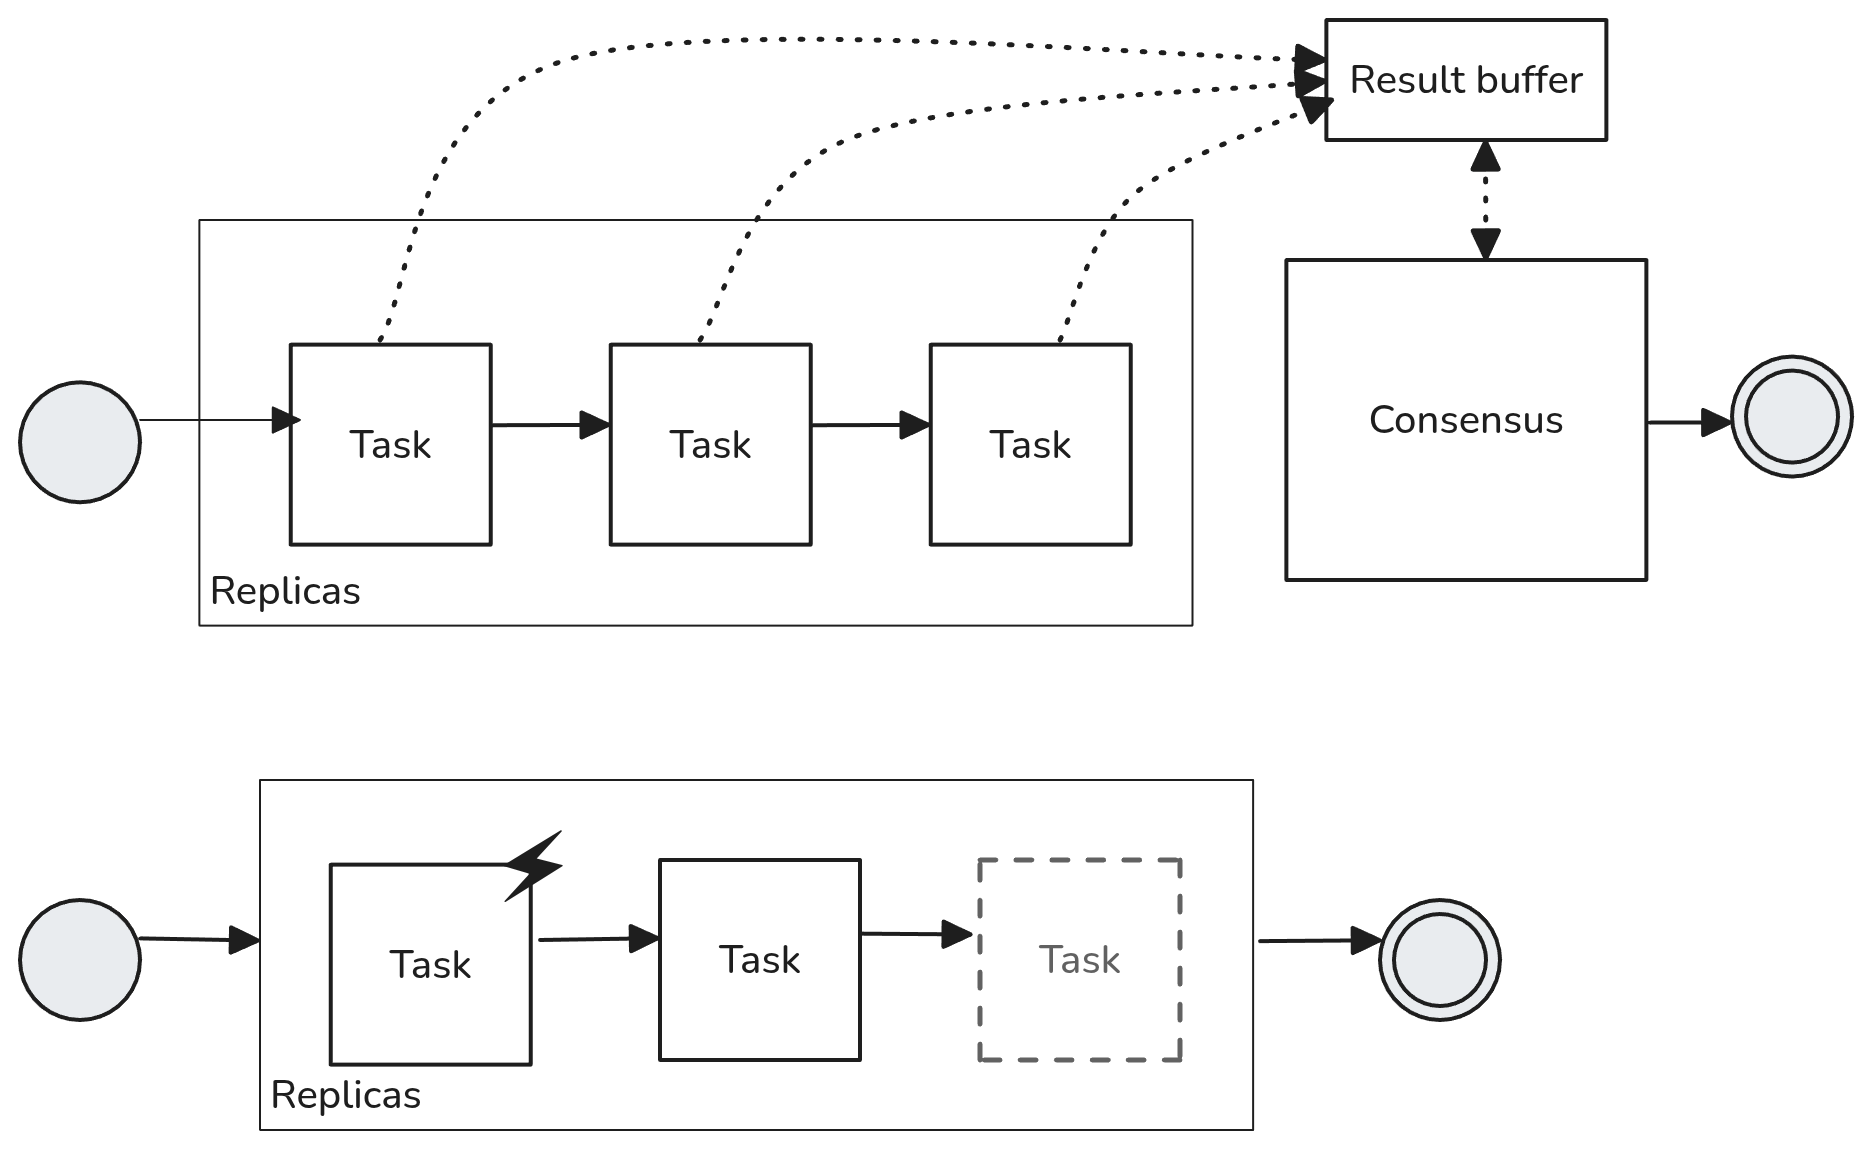
\includegraphics[width=1.0\textwidth]{assets/redundancia_reexec.png}
    \captionsetup{justification=raggedright}
    \caption*{Fonte: Elaborada pelo autor}
    \label{fig:redundanciaReexec}
\end{figure}

Na \autoref{fig:redundanciaReexec} é possível observar a reexecução de uma tarefa em duas modalidades: Na primeira é realizado um consenso entre os resultados das execuções, e na segunda a tarefa é apenas reexecutada até $N$ vezes (podendo então tolerar até $N$ falhas transientes), encerrando sua execução caso nenhuma falha seja detectada. A segunda modalidade é particularmente útil para a implementação de condições de transparência \cite{SchedAndOptOfDistributedFT} que serão abordadas posteriormente.

\subsubsection{Redundância}

Adicionar redundância ao sistema é uma das formas mais intuitivas e mais antigas de aumentar a tolerância à falhas, a probabilidade de $N$ falhas transientes ocorrendo simultaneamente em um sistema é mais baixa do que a probabilidade de apenas 1 falha \cite{SchedAndOptOfDistributedFT}.

Uma técnica de redundância comum é o uso de redundância modular, tipicamente com 3 instâncias replicadas (neste caso chamada de TMR ou "Triple Modular Redundancy"), a \autoref{fig:redundanciaTMR} ilustra a execução concorrente seguida de um votador.

O uso de TMR para uma tarefa pode consistir na reexecução concorrente das três instâncias, tendo seus resultados decidos por um votador. No contexto de tempo-real é importante que caso alguma das tasks no processo de execução concorrente viole sua deadline, que o votador ainda escolha um resultado para garantir o critério de tempo-real. O uso de TMR é elegante em sua simplicidade e consegue atingir um bom grau de resiliência, porém com o custo adicional de triplicar o custo em termos de memória e execução \cite{DependabilityInEmbeddedSystems}, e potencialmente necessitar de hardware mais poderoso para manter a mesma performance esperada.

\begin{figure}[H]
    \centering
    \captionsetup{justification=centering}
    \caption{Exemplo de execução com redundância}
    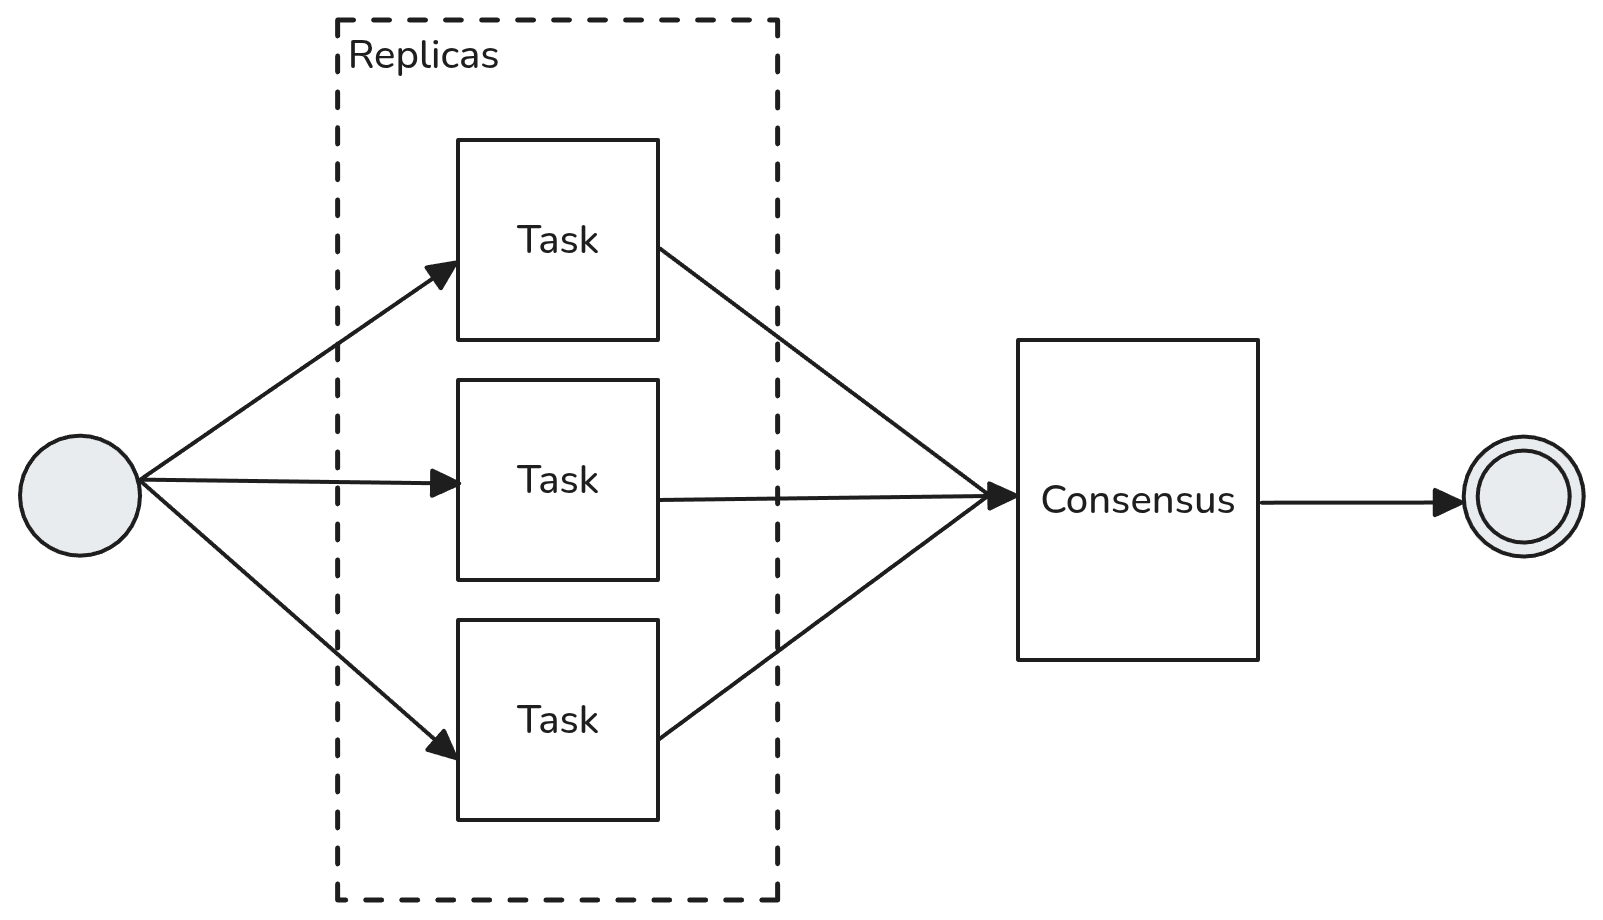
\includegraphics[width=1.0\textwidth]{assets/redundancia_tmr.png}
    \captionsetup{justification=raggedright}
    \caption*{Fonte: Elaborada pelo autor}
    \label{fig:redundanciaTMR}
\end{figure}

Sistemas distribuídos, sejam estes embarcados ou não, também podem aproveitar de sua redundância natural para ter maior dependabilidade \cite{MakingReliableDistSystems}. Falhas em um nó podem ser propagadas e no caso de falhas permanentes em um nó, os outros podem suplantar a execução de suas tarefas mantendo a qualidade média de serviço \cite{MakingReliableDistSystems} \cite{SchedAndOptOfDistributedFT}, o uso de sistemas capazes de auto reparo é vital para a existência de telecomunicação em larga escala e computação em nuvem.

\subsubsection{Loop Unrolling e Function Inlining}

Uma otimização comum que compiladores realizam é desenrolar laços de repetição (Loop Unrolling) com a finalidade de reduzir erros no preditor de desvios da CPU, no contexto de tolerância à falhas, é possível utilizar dessa otimização como uma forma de redundância espacial, ao reduzir a possibilidade de pulos dependentes de um valor, torna-se menos provável um salto baseado em uma versão corrompida do mesmo. O desenrolamento pode também ser feito caso exista um limite superior conhecido no laço durante a compilação. \cite{LoopUnrollingARM}.

Outra transformação comum é o inlining de funções, onde o corpo de uma função é copiado como se o código tivesse sido diretamente escrito em seu ponto de chamada. Ao reduzir a quantidade de pulos é possível melhorar a coerência do cache de instruções além de permitir outras otimizações durante os passes otimizantes do compilador \cite{EngineeringACompiler}, causando uma melhora na performance. No caso de tolerância à falhas, ao reduzir a quantia de jumps e prover redundância de instruções, o inlining pode também reduzir a chance de um salto inadequado \cite{MakingReliableDistSystems}. %TODO(marcos): citar aqui tbm

Importante ressaltar que aplicar \textit{function inlining} e \textit{loop unrolling} de forma excessiva pode resultar no oposto do que se deseja no quesito de performance, quando aplicadas de forma agressiva, essas otimizações saturam o cache de instruções, utilizam de mais registradores e ocupam espaço desnecessário no executável \cite{EngineeringACompiler}. Portanto, é importante que estas técnicas não sejam aplicadas de forma arbitrária e que seu uso seja acompanhado de medição para confirmar sua efetividade.

\subsection{Injeção de falhas}

Para adequadamente testar a dependabilidade do sistema, é possível deliberadamente causar falhas com o propósito de catalogar e validar se o sistema atinge as métricas necessárias. Dentre os tipos de teste que podem ser realizados, é possível categorizá-los em quatro grupos principais:

Injeção \textbf{Física}: Envolve utilizar um ambiente físico genuíno para causar as falhas, o principal benefício desta técnica é replicar eventos reais que possam causar falhas, assim como poder injetar falhas em superfícies reais do dispositivo \cite{FaultInjectionTechniques}. O principal problema é que esta técnica é particularmente cara e requer auxílio de equipamentos e profissionais especializados, também não é possível injetar um tipo específico de dado para testar um caso específico.

Injeção \textbf{Lógica em Hardware}: Utiliza-se de um dispositivo adicional para injetar as falhas que controla o dispositivo alvo, possui como vantagem ser menos intrusivo e ainda permitir um algo grau de controle e simulação dos fenômenos físicos, desvantagens incluem uma área maior de circuito necessária, implementação de uma unidade extra e criação de canais de comunicação com o dispositivo alvo \cite{FaultInjectionTechniques}.

Injeção \textbf{Lógica em Software}: Funções são executadas em software para injetar falhas em outras partes do programa, o método é pouco invasivo, de baixo custo, alta portabilidade e permite um controle muito elevado sobre os pontos de injeção e estilo de falha \cite{FaultInjectionTechniques}. Possui a desvantagem de aumentar o tempo médio de execução ao introduzir um custo extra de memória para armazenar o código de injeção, e nem sempre reproduz precisamente fenômenos físicos.

Injeção \textbf{Simulada}: O dispositivo é executado em um ambiente totalmente simulado, tem como vantagem não ser invasivo, altamente flexível e nem sequer necessitar de uma versão física do dispositivo, porém tipicamente requer software de simulação potencialmente caro assim como uma descrição do chip na forma de alguma linguagem de descrição de hardware, que raramente é disponibilizada \cite{FaultInjectionTechniques}.


\section{Sistemas embarcados}

Sistemas embarcados são uma família vasta de sistemas computacionais, algumas das principais características de sistemas embarcados são:

\textbf{Especificidade}: Diferente de um sistema de computação mais generalizado como um computador pessoal ou um servidor, sistemas embarcados são especializados para uma solução de escopo restrito. Exemplos de sistemas embarcados variam de microcontroladores encontrados em carros, televisões e dispositivos IoT até sistemas sofisticados de navegação de aeronaves e navios de grande porte \cite{ComputerOrganizationAndDesign}.

\textbf{Limitação de recursos}: Um corolário da natureza especialista destes sistemas, é que recursos alocados para o sistema são definidos previamente. No caso de microcontroladores o poder de processamento e quantidade de memória podem ser restritos para satisfazer uma necessidade de baixo custo de fabricação e menor consumo energético \cite{ComputerOrganizationAndDesign}. Importante notar que existem sistemas embarcados com acesso maior à recursos, como certos equipamentos de rede e aceleradores, mas os recursos do sistema continuam estaticamente delimitados para cumprir sua função específica.

\textbf{Critério Temporal}: Sistemas embarcados, por serem parte de um todo maior, devem realizar sua função com o mínimo de interrupção para a funcionalidade geral do contexto externo \cite{OperatingSystemConcepts}. A importância do tempo de execução de uma tarefa de um sistema pode ser classificada em duas principais categorias: Soft Real-Time , e Hard Real-Time , a distinção entre estas categorias é explicada na seção seguinte.

\subsection{Sistemas Operacionais de Tempo-Real}

Um sistema operacional é um conjunto de software que permite o gerenciamento e interação com os recursos do hardware através de uma camada de abstração. O componente essencial de um sistema operacional é o kernel, que sempre está executando, A função primordial do kernel é viabilizar a coexistência de diversas tarefas no sistema, as quais demandam acesso às capacidades do hardware, notadamente o tempo de processamento da CPU e o espaço de memória. De forma simplificada, o kernel pode ser descrito como a "cola" entre as aplicações e os recursos de hardware \cite{OperatingSystemConcepts}.

Um sistema operacional de tempo real (RTOS) é um tipo de sistema operacional mais especializado, tipicamente pequeno, que possui como característica central cumprir um critério temporal Real-Time , que é dividido em 2 categorias:

\begin{itemize}
    \item \textbf{Soft Real-Time }: Um sistema que garante essa propriedade precisa sempre garantir que tarefas de  maior importância tenham prioridade sobre as de menor importância. Sistemas Soft Real-Time  tipicamente operam na escala de milissegundos, isto é, percepção humana \cite{SchedAndOptOfDistributedFT}. O atraso de uma tarefa em um sistema Soft Real-Time  não é desejável, mas não constitui uma falha. Exemplos: Player de DVD, videogames, kiosks de atendimento automáticos.
    
    \item \textbf{Hard Real-Time }: Precisam garantir as propriedades de Soft Real-Time , além disso, o atraso de uma tarefa de seu prazo, é inaceitável, para um sistema Hard Real-Time  uma resposta com atraso é o mesmo que resposta nenhuma. Cuidado adicional deve ser utilizado ao projetar sistemas Hard Real-Time , pois muitas vezes aparacem em contextos críticos \cite{ModernOperatingSystems}. Exemplos: Software para sistema de frenagem, sistemas de navegação em aplicações aeroespaciais, software de negociação de alta frequência, fila de mensagens de alta performance
\end{itemize}

Como sistemas que cumprem o critério Hard Real-Time também cumprem os requisitos Soft Real-Time, os sistemas operacionais de tempo real tipicamente tem sua arquitetura orientada a serem capazes de cumprir o critério Hard Real-Time  \cite{SchedAndOptOfDistributedFT}.

Diferentemente de sistema operacionais focados em uso geral como Windows, Linux e OSX, os RTOSes não priorizam fornecer ao usuário uma sensação de fluidez e adaptabilidade. Devido à seus requisitos temporais rígidos, um RTOS é feito com um foco significativo em determinismo, confiabilidade e simplicidade, para garantir que tarefas sejam executadas com um respeito estrito de seus prazos \cite{OperatingSystemConcepts}. Exemplos de RTOS disponíveis no mercado incluem: FreeRTOS, VxWorks, Zephyr e LynxOS.

\subsection{Escalonador}

O escalonador é o componente do sistema operacional responsável por gerenciar múltiplas tarefas que desejam executar \cite{OperatingSystemConcepts}, sendo um componente extramente crucial, a implementação do escalonador deve garantir que tarefas de alta prioridade executem antes e que a a troca de contexto seja o mais rápido possível. O algoritmo de escalonamento é o fator central para o comportamento do escalonador, sendo categorizados em dois princpais grupos:

\begin{itemize}
    \item \textbf{Cooperativos}: Tarefas precisam voluntariamente devolver o controle da CPU (com exceção de certas interrupções de hardware) para que as outras tarefas possam executar, isso pode ser feito explicitamente por uma função de largar ou implicitamente ao utilizar uma rotina assíncrona do sistema, como ler arquivos, receber pacotes de rede ou aguardar um evento \cite{OperatingSystemConcepts}.

    \item \textbf{Preemptivos}: Além de poderem transferir a CPU manualmente, o escalonador forçará trocas de contexto caso uma condição para a troca seja satisfeita. O algoritmo mais comum que serve de base para diversos escalonadores preemptivos é o Round-Robin onde tarefas possuem uma quantia de tempo máximo alocada para sua execução contínua, nomeada "fatia de tempo" ou "quantum" \cite{ModernOperatingSystems}. Tarefas ainda podem possuir relações de prioridade, alterando a ordem que o escalonador realiza seu despache assim como o tamanho de sua fatia de tempo.
\end{itemize}

Sistemas operacionais de tempo real são tipicamente executados no modo totalmente preemptivo, mas o uso cooperativo também é viável e possui a vantagem de possuir um controle mais granular da execução das tarefas, mas é importante que seja tomado o cuidado adequado para que nenhum prazo de execução Hard Real-Time seja violado por uma tarefa inadvertidamente utilizando a CPU por uma quantidade longa de tempo.

\subsection{Concorrência e Assincronia}

Será utilizado a definição de concorrência como a habilidade de um sistema de lidar com múltiplas tarefas computacionais dividindo seus recursos (particularmente tempo de CPU e memória). Isto é, um sistema não necessariamente precisa ser paralelo (execuções múltiplas simultâneas) para possuir concorrência, mas para tornar paralelismo viável, o sistema necessita de mecanismos de concorrência \cite{MakingReliableDistSystems}.

Uma característica central para a utilidade de concorrência mesmo em situações em que paralelismo é limitado ou impossível vai além da pura expressividade do programador, existem assimetrias grandes na velocidade de acesso de disco, memória, rede, e caches da CPU como demonstrado na \autoref{fig:latencia}. Para acessar recursos de forma eficaz, é necessário lidar com suas características inerentemente assíncronas. O uso de concorrência permite que uma tarefa seja suspensa e resumida (voluntariamente ou não) o que permite que o sistema não fique excessivamente ocioso \cite{OperatingSystemConcepts}.

\begin{figure}[H]
    \centering
    \captionsetup{justification=centering}
    \caption{Hierarquia de latência de acessos}
    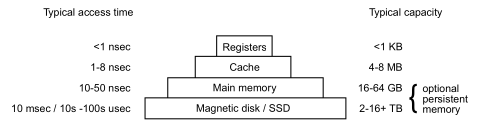
\includegraphics[width=1.0\textwidth]{assets/latency_hierarchy.png}
    \captionsetup{justification=raggedright}
    \caption*{Fonte: \figcite{ModernOperatingSystems}}
    \label{fig:latencia}
\end{figure}

Implementar os mecanismos de concorrência adequados também permite lidar com interrupções de forma mais estruturada, um problema clássico de lidar com uma interrupção é restaurar a memória de pilha e registradores de forma adequada, interrupções introduzem um fluxo de programa não local
%TODO livro de iface e impl em c
, violando as garantias fortes de escopo e ponto de entrada fornecidas por funções.

É uma tendência atual aumentar o número de núcleos em dispositivos, com velocidades de relógio das CPUs possuindo ganhos marginais em relação ao impacto térmico, a maioria dos computadores de propósito geral (smartphones, tablets, desktops) tipicamente possuem 2 núcleos ou mais \cite{ComputerOrganizationAndDesign}. Essa tendência não se restringe apenas à computadores gerais, sistemas embarcados comerciais também podem se beneficiar tremendamente das possibilidades de concorrência providas por mais de um núcleo, porém, é importante ressaltar que o uso de estado compartilhado se torna muito mais sensível à erros em um ambiente com múltiplos fluxos de execução, e medidas devem ser tomadas para evitar condições de corridas e deadlocks \cite{OperatingSystemConcepts}.

\subsection{Grafos de Processos tolerantes à falhas}

Para uma representação mais clara e eficaz de um fluxo de execução sujeito a falhas, é possível utilizar de grafos resilientes a falhas como um mecanismo de diagramação. Nesta representação, os nós correspondem a tarefas, as quais podem ser executadas na mesma unidade de processamento ou não. As arestas do grafo representam o fluxo de execução, uma aresta não demarcada indica execução incondicional, enquanto arestas demarcadas com notação de mensagem designam uma execução condicional à transmissão de uma mensagem. Mensagens e tarefas representadas por símbolo circular indicam pontos ordinários no grafo, ao passo que símbolos quadrados denotam condições de transparência. \cite{SchedAndOptOfDistributedFT}.

Um grafo de processos tolerantes é falhas é definido como um grafo não ponderado direcionado acíclico com seus nós representando tarefas/processos, arestas representam o fluxo de execução e arestas nomeadas representam fluxo dependente da entrega de mensagens. Será utilizado a notação $P_X (N)$, onde $X$ é o número identificador da tarefa, e $N$ corresponde à sua $N$-ésima re-execução, por exemplo: $P_2 (1)$ indica a primeira execução da tarefa $P_2$, enquanto $P_1 (3)$ indica a terceira reexecução da tarefa $P_1$. Uma notação similar será utilizada para mensagens entre tarefas, $m_X (N)$, mensagens, assim como tarefas, estão sujeitas à falhas e custos adicionais de detecção, mas ao invés de re-execução, mensagens são re-enviadas \cite{SchedFTWithSoftAndHardConstraints}.

Para melhor exemplificar a importância da detecção das falhas, será tomado como exemplo um grafo simples, com apenas 3 tarefas e uma mensagem. O grafo precisará tolerar uma falha transiente. O fluxo "ideal" é demonstrado na \autoref{fig:ftgSimples}.

\begin{figure}[H]
    \centering
    \captionsetup{justification=centering}
    \caption{Grafo com 3 processos e uma mensagem}
    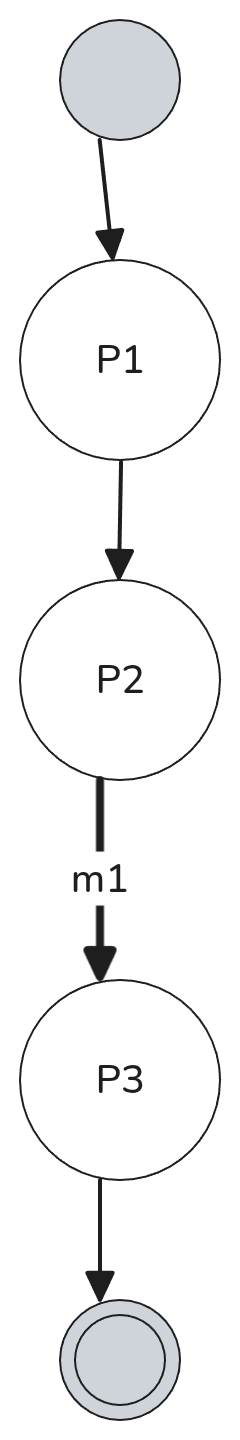
\includegraphics[width=0.120\textwidth]{assets/ftg_simples.png}
    \captionsetup{justification=raggedright}
    \caption*{Fonte: Elaborada pelo autor}
    \label{fig:ftgSimples}
\end{figure}

Ao incluir os diferentes desvios possíveis na presença de apenas uma falha, o grafo de execução da \autoref{fig:ftgExpandido} é obtido. A incidência de falhas no processamento ou passagem de mensagens é indicada com um ícone de raio.

\begin{figure}[H]
    \centering
    \captionsetup{justification=centering}
    \caption{Mesmo grafo, mas tolerante à uma falha transiente}
    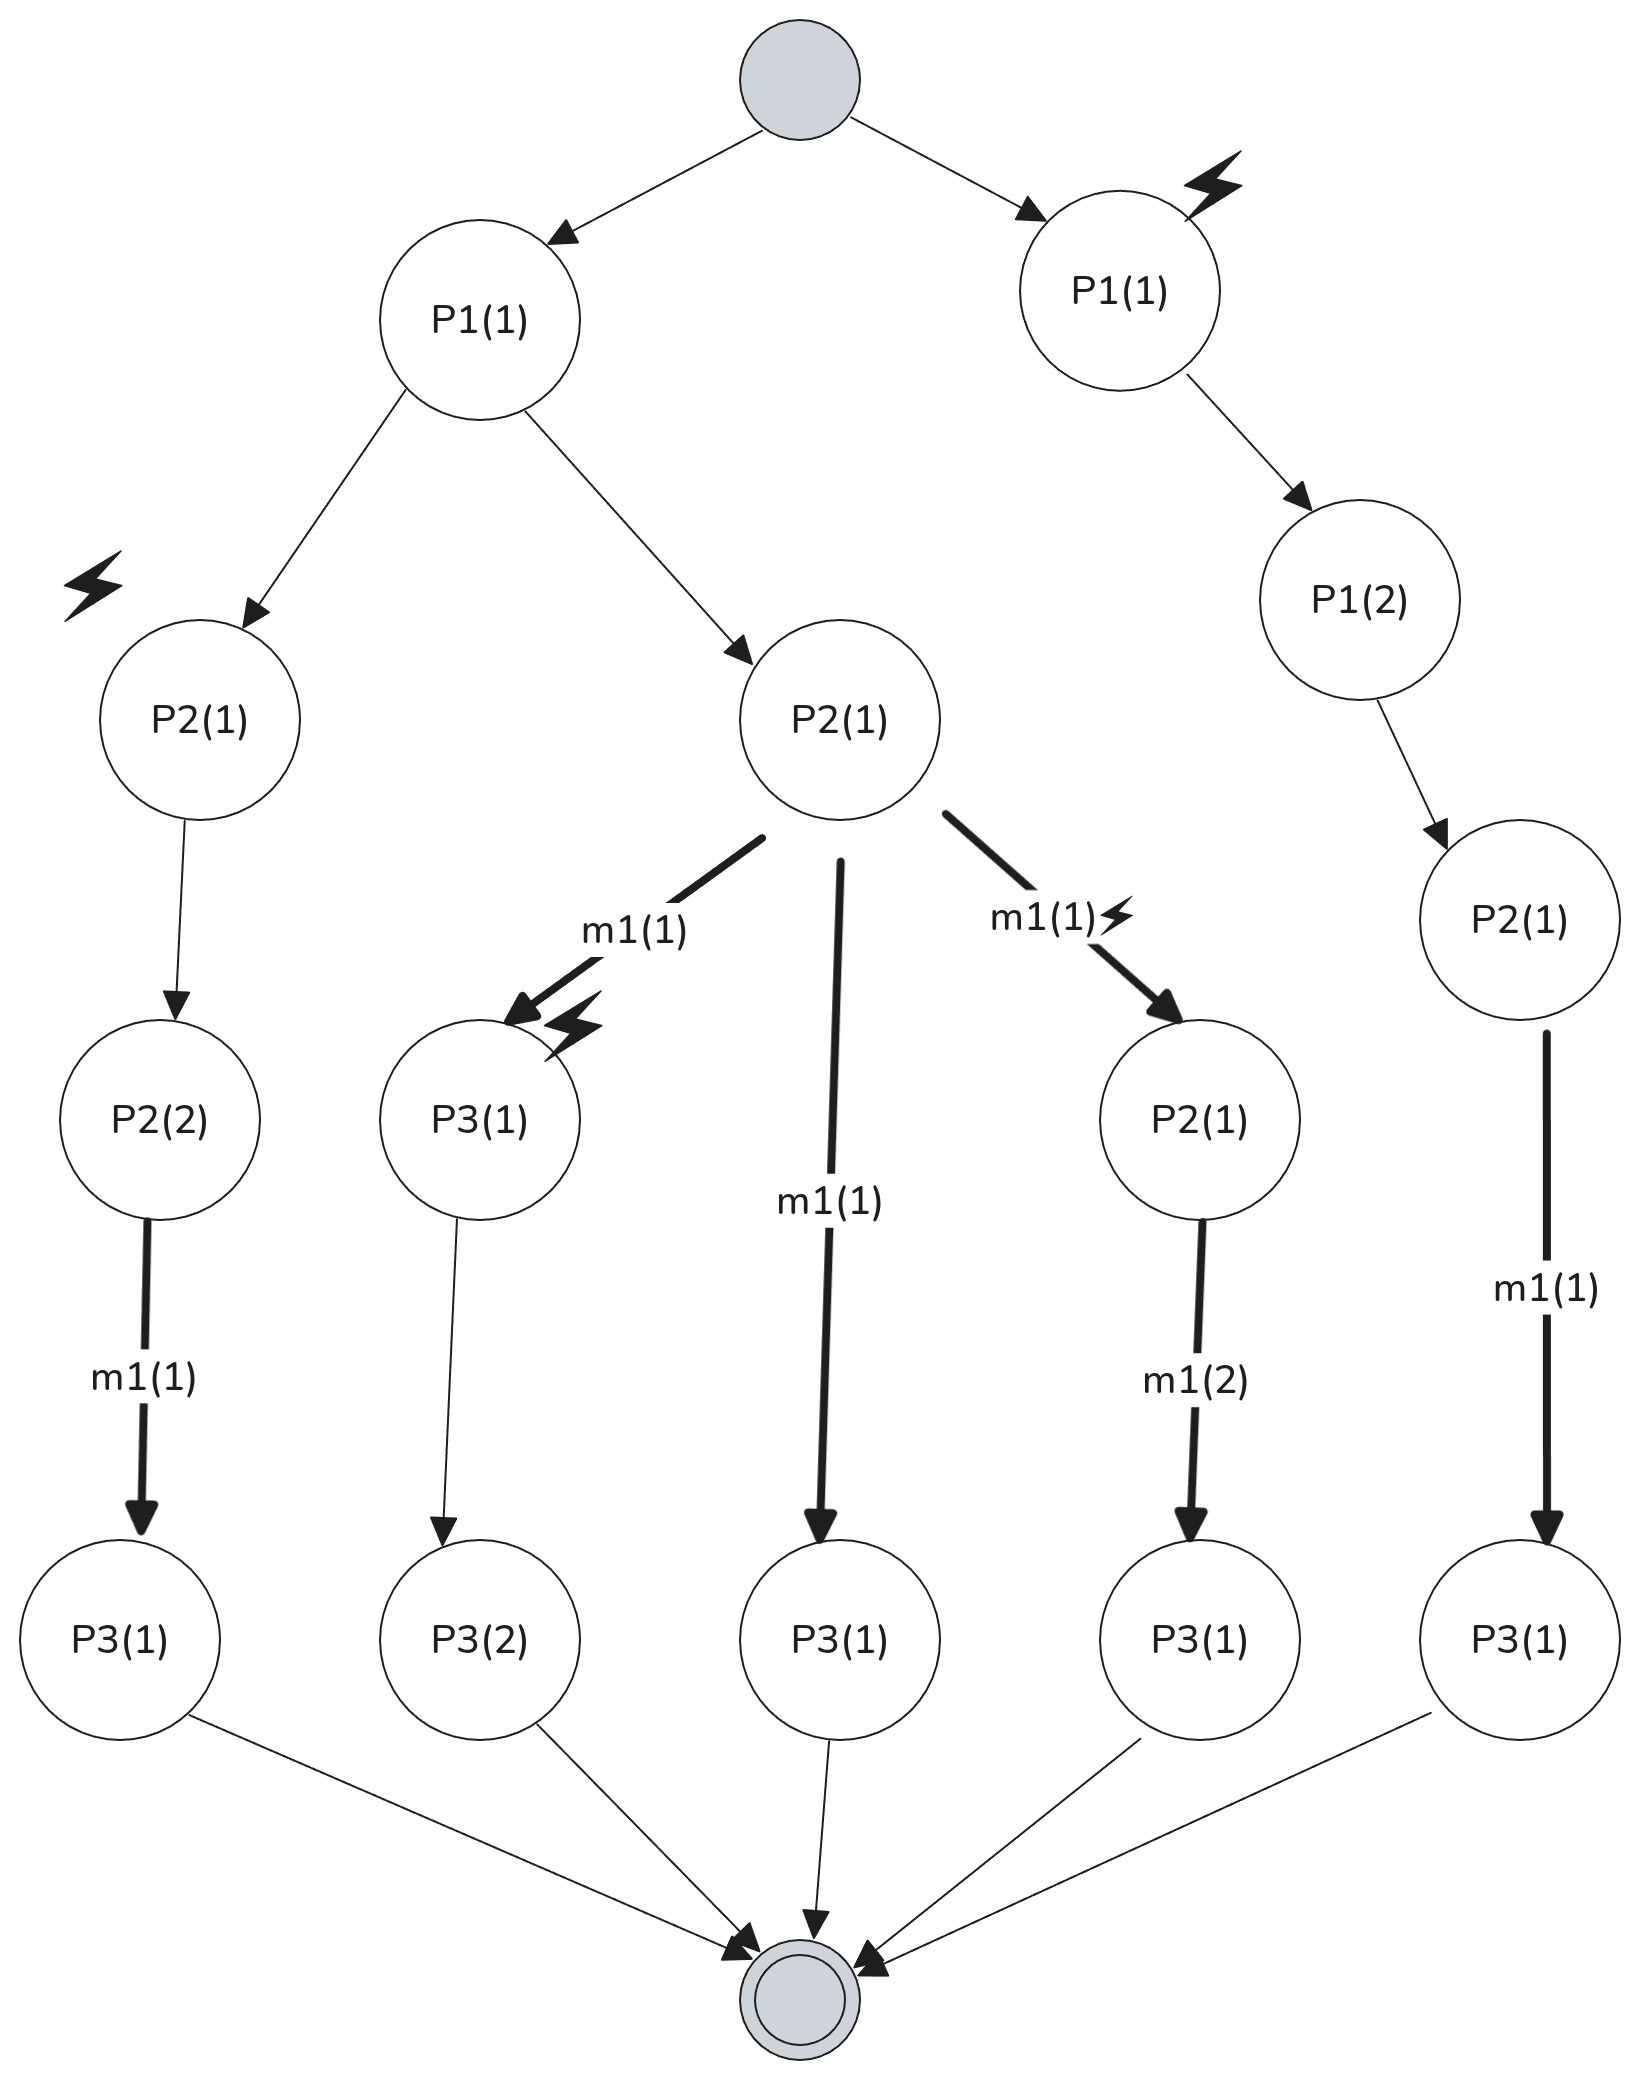
\includegraphics[width=0.75\textwidth]{assets/ftg_expandido.png}
    \captionsetup{justification=raggedright}
    \caption*{Fonte: Elaborada pelo autor}
    \label{fig:ftgExpandido}
\end{figure}

Será introduzido transparência na tarefa $P_2$, isto é, será executada com redundância temporal ou modular de tal forma que as tarefas subsequentes pudessem assumir "como se" uma falha nunca tivesse acontecido em $P_2$ após sua deadline ter sido completa, o grafo na \autoref{fig:ftgTransparencia} demonstra a condição de transparência com um ícone retangular.

\begin{figure}[H]
    \centering
    \captionsetup{justification=centering}
    \caption{Introdução de transparência em $P_2$}
    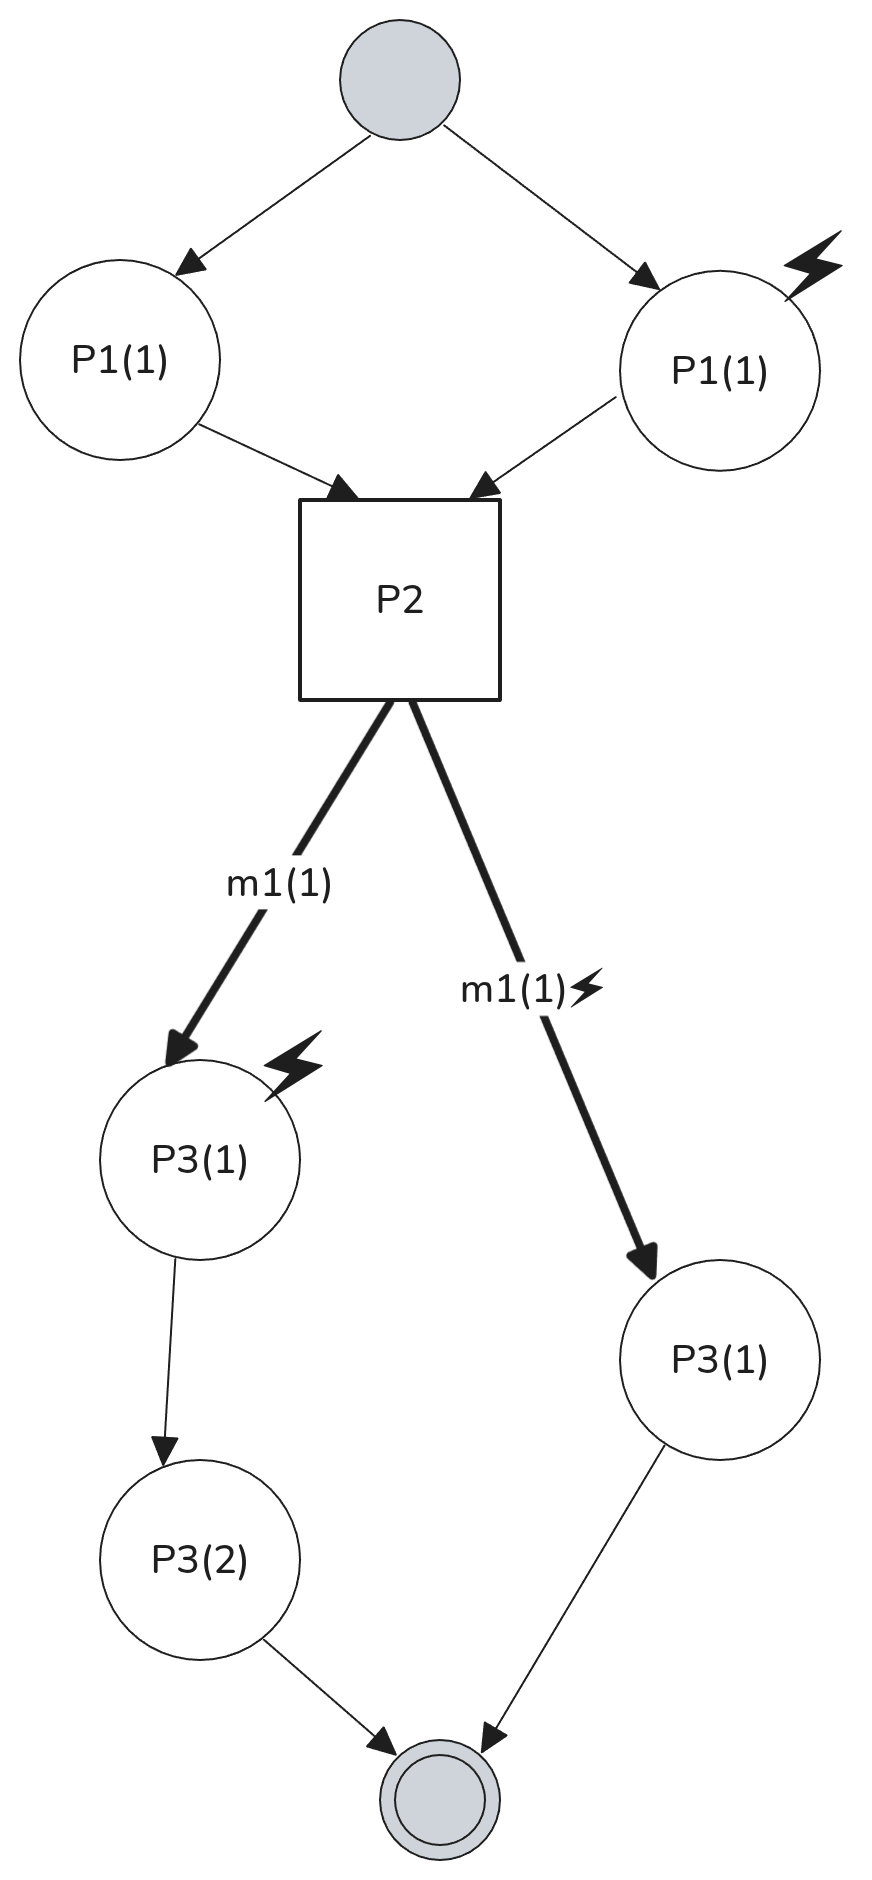
\includegraphics[width=0.40\textwidth]{assets/ftg_transparencia.png}
    \captionsetup{justification=raggedright}
    \caption*{Fonte: Elaborada pelo autor}
    \label{fig:ftgTransparencia}
\end{figure}

Introduzindo apenas um ponto de transparência é possível reduzir significativamente as possibilidades de execução do sistema, isso é particularmente benéfico para escalonadores ou algoritmos de tratamento de falhas baseados em máquinas de estado finito. Um grafo mais compacto é benéfico a previsibilidade do sistema, estabelecendo uma relação forte de pré-conclusão com sucesso ao respeitar o prazo da tarefa transparente \cite{SchedAndOptOfDistributedFT}.

Este exemplo é simples e tolera apenas uma falha transiente, porém processos complexos com múltiplas mensagens entre si causam um aumento exponencial de complexidade, especialmente caso seja necessário tolerar até $k$ falhas transientes.

Pode-se adicionar pontos de transparência através de reexecução ou redundância modular (se a deadline conjunta das $N$ tarefas for determinística) para aumentar a confiabilidade e previsibilidade do sistema. Essa transparência não é gratuita: há um troca entre maior confiabilidade no escalonador e menor imprevisibilidade na execução, com o custo de maior uso de CPU e memória. Todos os pontos precisam ser verificados, o que pode aumentar o tempo ocioso dos núcleos e exigir a extensão do prazo da tarefa para permitir reexecuções suficientes.

\section{Trabalhos relacionados} \label{sec:trabRel}
\subsection{Técnica de confiabilidade em nível de sistema operacional para a arquitetura RISC-V}

\indirectcite{TecnicaConfiabilidadeRISCV}

\subsection{Reliability Assessment of Arm Cortex-M Processors under Heavy Ions and Emulated Fault Injection}

Neste trabalho conjunto de pesquisadores da USP e UFRGS utilizam de um sistema COTS e criam um perfil de falhas com exposição a íons pesados assim como injeção artificial de falhas para posteriormente realizar uma adição de formas de detecção de falhas para melhorar a confiabilidade do sistema. Foi possível detectar mais da metade das falhas funcionais apenas com técnicas de software no banco de registradores. \cite{ReliabilityArmCortexUnderHeavyIons}.

% TODO: referenciar a imagem
\begin{figure}[H]
    \centering
    \captionsetup{justification=centering}
    \caption{Análise de resiliência, dividida por categoria}
    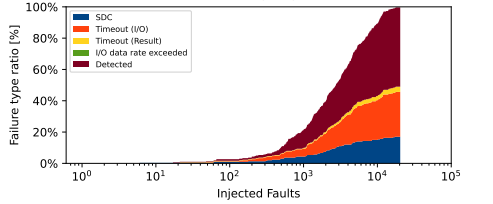
\includegraphics[width=0.75\textwidth]{assets/related_works_heavy_ion_reliability.png}
    \captionsetup{justification=raggedright}
    \caption*{Fonte: \figcite{ReliabilityArmCortexUnderHeavyIons}}
    \label{fig:trabRelIonsPesados}
\end{figure}

Uma outra observação foi que a quantia de falhas injetadas para ocasionar um erro de funcionalidade é 2 ordens de magnitude maior na memória em relação ao banco de registradores, indicando que existe uma necessidade real de poder detectar e mitigar erros de memória mais rapidamente \cite{ReliabilityArmCortexUnderHeavyIons}.

\subsection{Application-Level Fault Tolerance in Real-Time Embedded System}

Neste trabalho são apresentadas técnicas de tolerância à falhas em um sistema operacional chamado BOSS, é utilizado uma interface de thread com a implementação de tolerância conformando à interface. O trabalho naturalmente explora o escalonador mas não entra em detalhamento profundo na parte de detecção, mas sim de prover uma biblioteca na forma de classes representando threads resilientes \cite{ApplicationLevelFT}. Um caso de estudo de um sistema de filtragem de radar é utilizado como projeto.

Os pesquisadores demonstraram resultados favoráveis para uma forma híbrida de tolerância com menor uso de CPU em relação à redundância tripla utilizando de técnicas em software combinado com um par de processadores com auto checagem (PSP).

% TODO: referenciar a imagem
% #sourced_image(
% 	caption: [Utilização de CPU para diferentes implementações de tolerância],
% 	source: "ApplicationLevelFT",
% 	image("assets/related_works_psp_perf.png"),
% )

O trabalho demonstra também a viabilidade de prover interfaces mais abstratas que ainda sejam capazes de rodar em sistemas de recursos restritos.

\subsection{Análise Comparativa dos trabalhos relacionados}



% \renewcommand{\arraystretch}{1}
%  \begin{quadro}[H]
%     \centering
%     \caption{Comparação de trabalhos relacionados}
%     \label{tab:trabrel}
%     \begin{tabular}{|m{0.126\textwidth}|m{0.135\textwidth}|m{0.10\textwidth}|m{0.115\textwidth}|m{0.11\textwidth}|m{0.18\textwidth}|}
%         \hline
%         \rowcolor[HTML]{C0C0C0}
%         \textbf{Trabalho}  & \textbf{CNN base} & \textbf{Imagem} & \textbf{Tipo de Resolução} & \textbf{$\mu$C} & \textbf{Métricas} \\ \hline
        
%         \Centering\textbf{\citeDir{azami2022earth}}  & ShallowNet, LeNet e MiniVGGNet & RGB & Espacial e Espectral & Raspberry Pi 3+ & Acurácia \\ \hline
        
%         \Centering\textbf{\citeDir{maskey2020cubesatnet}}  & CubeSatNet & RGB & Espacial e Espectral & STM32H & Acurácia Global, \textit{F1-score} e Memória \\ \hline 
        
%         \Centering\textbf{\citeDir{leong2021unet}}  & U-net & RGB & Espacial e Espectral & STM32F7 & Precisão, Sensibilidade, Falso Negativo, Falso Positivo, Acurácia Global, \textit{F1-score} e Memória \\ \hline
        
%         \Centering\textbf{Este trabalho}  & LeNet-5 e HybridSN & HSI & Espectral & ESP32 e/ou Raspberry Pi Pico & Acurácia, F1-Score, Sensibilidade, Tempo de Processamento, Memória Utilizada, Potência Dissipada e Energia Consumida\\ \hline
%     \end{tabular}
%  \end{quadro}
%  \renewcommand{\arraystretch}{1}
 
